%!TeX spellcheck = en_US
\documentclass[12pt,a4paper,USenglish]{article}      % Specifies the document class
\usepackage[utf8]{inputenc}
\usepackage[T1]{fontenc,url}
\usepackage{babel,csquotes,newcent,textcomp}
\usepackage[backend=biber,sortcites]{biblatex}
\usepackage{graphicx}
%\usepackage{listings}
\usepackage{comment}

\usepackage{listings}
\usepackage{color}

\definecolor{dkgreen}{rgb}{0,0.6,0}
\definecolor{gray}{rgb}{0.5,0.5,0.5}
\definecolor{mauve}{rgb}{0.58,0,0.82}

\lstset{frame=tb,
  language=Java,
  aboveskip=3mm,
  belowskip=3mm,
  showstringspaces=false,
  columns=flexible,
  basicstyle={\small\ttfamily},
  numbers=left,
  numberstyle=\tiny\color{gray},
  keywordstyle=\color{blue},
  commentstyle=\color{dkgreen},
  stringstyle=\color{mauve},
  breaklines=true,
  breakatwhitespace=true,
  tabsize=3
}

\graphicspath{ {./images/} }

\addbibresource{References.bib}
\title{Methodology}  % Declares the document's title.
%\newcommand{\ip}[2]{(#1, #2)}

\begin{document}             % End of preamble and beginning of text.
%\maketitle                   % Produces the title.
\section{Benchmarks}
%There are four different benchmarks.
\subsection{Introduction}
Persistence memory is slower than DRAM. But there is not much information on how much slower the NVDIMM is in comparison to DRAM. This chapter will test the performance of NVDIMM when it work alone and when it works simultaneously with DRAM. The results will be presented with graphs and tables that will show the difference in performance.
The chapter will start off with using the STREAM\cite{STREAM-c} benchmark in to find the performance of DRAM.
The NVDIMM will also be tested with a STREAM benchmark that have been modified by the author of this thesis. 
Three original benchmarks will also test the NVDIMM when it works simultaneously with DRAM.
In the first benchmark DRAM will copy an array from DRAM-DRAM while NVDIMM copy and array from NVDIMM-NVDIMM. In the second benchmark DRAM will copy from DRAM-DRAM while NVDIMM will copy from NVDIMM-DRAM. In the last benchmark DRAM will copy from DRAM-DRAM while NVDIMM will copy from DRAM-NVDIMM.

\subsubsection{Hardware}
The program have been tested on a server with the following hardware.\\
Motherboard: Supermicro X11DPU-Z+ \\
CPU: Intel(R) Xeon(R) Gold 6130 CPU @ 2.10GHz, 16 cores \\
DRAM: Samsung RDIMM, 2666 MT/s. \\
NVDIMM: Micron Technology NV-DIMM , 2933 MT/s \\
\\
The server have two CPU, both CPU have twelve memory slots each. Each CPU have six channels. There are one DRAM and one NVDIMM sharing one channel.
The compiler used to compile the code is gcc (Ubuntu 7.5.0-3ubuntu1~18.04) 7.5.0. The code have been optimized to level two.

All of the benchmarks have been tested on socket two. This is to avoid disturbances as much as possible since most of the other processes are running on socket one

\subsection{STREAM DRAM}
\label{section:STREAMDRAM}
The STREAM\cite{STREAM-c} benchmark is a synthetic and simple benchmark that is designed to measure bandwidth in MB/s. This benchmark is seen as the standard for measuring memory bandwidth and has not been modified in any way after it was downloaded from the creators websites.
The benchmark test memory bandwidth by running four different tests. The first one test is copy where the elements in one array is copied to another array.
The second test is called scale where each element are multiplied with a constant and the result is placed in a second array, the index of the element in the first array and the result in the second array is the same.
Third test is add where the elements from two different arrays with the same index are added together and place in a third array where the index is the same as in the two other arrays.
Last test is the triad where the one array is multiplied with a constant then added together with a second array and then placed in a third array.

The DRAM Stream benchmark run the test 32 times and only on one socket, every times it restart with one extra thread is added. The CPU has 16 cores and when the thread number surpass that number it starts using the hyper thread on the same core. The Linux program numactl is also used to manage the number of threads and what socket the benchmark is allowed to used.

The result shown in figure \ref{fig:DRAM_STREAM_100M_Figure} and table \ref{tab:DRAM_STREAM_100M_Table} is what was expected, adding more threads in beginning will give a big increase in transfer speed. But at thread 5 there gains in transfer speed will start to diminish and at thread 11 there will be very little increase in transfer speed when adding more threads.
This means that it might be possible to allocate five of the sixteen threads to work on NVDIMM and not loose a significant amount of performance for the eleven remaining threads that are still working on DRAM. 

After sixteen threads the benchmark start to use the hyper-threads. There is a 10,000 MB/s decrease when the benchmark start to use the hyper-threads. When more and more hyper-threads are added the bandwidth will increase until it is almost at the same level when there was only sixteen threads. 32 threads have 2,000 MB/s lower bandwidth than sixteen threads.

\begin{figure}[!hbtp]
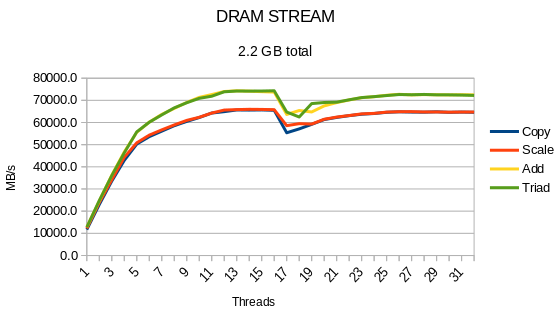
\includegraphics[scale=0.7]{Benchmarks/DRAM_STREAM_100M_Figure.png}
\caption{DRAM Stream, 100,000,000 elements}
\label{fig:DRAM_STREAM_100M_Figure}
\end{figure}

\begin{table}[!hbtp]
\begin{tabular}{ |c|c|c|c|c| }
\hline
Threads & Copy & Scale & Add & Triad \\
\hline
1 & 11673.5 & 12180.6 & 12799.4 & 12745.3 \\
\hline
2 & 22995.1 & 23892.4 & 24637.1 & 24807.8 \\
\hline
3 & 33554.9 & 34206.9 & 36248.9 & 36070.7 \\
\hline
4 & 42917.3 & 44315.0 & 46759.0 & 46333.7 \\
\hline
5 & 50260.9 & 50853.1 & 55574.9 & 55784.3 \\
\hline
6 & 53612.5 & 54305.3 & 60174.4 & 60129.4 \\
\hline
7 & 56100.8 & 56671.2 & 63670.6 & 63425.1 \\
\hline
8 & 58554.6 & 58888.6 & 66348.1 & 66607.5 \\
\hline
9 & 60491.7 & 60947.7 & 69059.1 & 68923.9 \\
\hline
10 & 62242.2 & 62368.3 & 71335.2 & 70900.6 \\
\hline
11 & 64257.1 & 64270.1 & 72604.0 & 71854.1 \\
\hline
12 & 64890.3 & 65611.6 & 73973.6 & 73866.7 \\
\hline
13 & 65648.8 & 65805.9 & 74285.3 & 74204.8 \\
\hline
14 & 65606.5 & 65943.6 & 74128.9 & 74158.9 \\
\hline
15 & 65665.5 & 65897.7 & 73918.8 & 74199.9 \\
\hline
16 & 65509.8 & 65770.4 & 73721.2 & 74312.2 \\
\hline
17 & 55365.3 & 58578.1 & 63624.8 & 64728.6 \\
\hline
18 & 57104.2 & 59481.5 & 65404.0 & 62472.2 \\
\hline
19 & 59160.6 & 59279.3 & 64749.4 & 68522.2 \\
\hline
20 & 61328.6 & 61453.3 & 67489.5 & 69020.7 \\
\hline
21 & 62290.7 & 62453.6 & 68987.6 & 69178.2 \\
\hline
22 & 63091.2 & 63146.4 & 70173.6 & 70239.2 \\
\hline
23 & 63737.2 & 63887.6 & 71195.5 & 71235.8 \\
\hline
24 & 64056.6 & 64108.0 & 71629.1 & 71669.4 \\
\hline
25 & 64601.7 & 64685.7 & 72282.9 & 72167.3 \\
\hline
26 & 64824.5 & 64850.8 & 72729.4 & 72623.9 \\
\hline
27 & 64706.3 & 64890.3 & 72444.1 & 72525.6 \\
\hline
28 & 64654.6 & 64743.1 & 72586.7 & 72656.9 \\
\hline
29 & 64827.0 & 64750.6 & 72505.7 & 72481.2 \\
\hline
30 & 64589.2 & 64659.6 & 72453.0 & 72472.8 \\
\hline
31 & 64703.8 & 64714.4 & 72531.8 & 72356.7 \\
\hline
32 & 64610.4 & 64721.9 & 72459.3 & 72212.9 \\
\hline
\end{tabular}
\caption{DRAM Stream, 100,000,000 elements}
\label{tab:DRAM_STREAM_100M_Table}
\end{table}

%\clearpage
\subsection{STREAM NVDIMM}
\label{section:STREAM_NVDIMM}
The stream NVDIMM benchmark measure the memory speed of the NVDIMM. This benchmark is the same as the STREAM benchmark has been descibed in chapter \ref{section:STREAMDRAM}. The different is that the memory type have been changed from DRAM to NVDIMM.
The code shown in listing \ref{lst:orgStreamDram} is part of the original code that have been removed from the code.
\begin{lstlisting}[caption={Original STREAM benchmark code at line 175-181.}, label={lst:orgStreamDram}]
#ifndef STREAM_TYPE
#define STREAM_TYPE double
#endif

static STREAM_TYPE  a[STREAM_ARRAY_SIZE+OFFSET],
                    b[STREAM_ARRAY_SIZE+OFFSET],
                    c[STREAM_ARRAY_SIZE+OFFSET];
\end{lstlisting}
It has been replaced with the code shown in listing \ref{lst:orgStreamNvdimm}. The code starts by opening the memory pool at line 21-27. The code will use a method called initiate at line 28 that will initiate the three arrays. Once this is done the code will continue executing the rest of the STREAM benchmark code which is identical to the original STREAM benchmark code.
\begin{lstlisting}[caption={Code that has replaced original code.}, label={lst:orgStreamNvdimm}]
PMEMobjpool *pop;
POBJ_LAYOUT_BEGIN(array);
POBJ_LAYOUT_TOID(array, double);
POBJ_LAYOUT_END(array);
//Declearing the arrays
TOID(double) a;
TOID(double) b;
TOID(double) c;

void initiate()
{
	//Initiating the arrays.
	POBJ_ALLOC(pop, &a, double, (STREAM_ARRAY_SIZE+OFFSET)*sizeof(STREAM_TYPE), NULL, NULL);
	POBJ_ALLOC(pop, &b, double, (STREAM_ARRAY_SIZE+OFFSET)*sizeof(STREAM_TYPE), NULL, NULL);
	POBJ_ALLOC(pop, &c, double, (STREAM_ARRAY_SIZE+OFFSET)*sizeof(STREAM_TYPE), NULL, NULL);
}

int main()
{
	const char path[] = "/mnt/pmem0-xfs/pool.obj";
	pop = pmemobj_create(path, LAYOUT_NAME, 10737418240, 0666);
	if (pop == NULL)
		pop = pmemobj_open(path, LAYOUT_NAME);
	if (pop == NULL) {
		perror(path);
		exit(1);
	}
	initiate();
	//The rest of the STREAM benchmark after this.
}
\end{lstlisting}

The result on NVDVIMM Stream benchmark shown in figure \ref{fig:NVM_STREAM_100M_Figure} and table \ref{tab:NVM_STREAM_100M_Table} is very different from the DRAM Stream benchmark. The the DRAM Stream benchmark had a steep increase in bandwidth in the beginning that started to taper off at thread five and almost no increase from thread eleven. The NVDIMM have a more linear increase in bandwidth when the threads are increased from one threads towards sixteen threads. 
This might be because the speed of one thread is half the bandwidth of one thread in the DRAM Stream benchmark. 
The max bandwidth reached by the NVDIMM Stream benchmark is 51,273 MB/s and the DRAM Stream benchmark start to taper off at around 55,000 MB/s. The NVDIMM Stream benchmark never reach a speed high enough so it can start to taper off and therefore it look more like linear increase in bandwidth.

Thread seventeen and after are the hyper-threads and at thread seventeen there is a 15,000 MB/s decrease before the bandwidth overall start to increase with more hyper-threads added. The bandwidth swing up and down a lot. There is no evidence on why the bandwidth fluctuate so much. 

\begin{figure}[!hbtp]
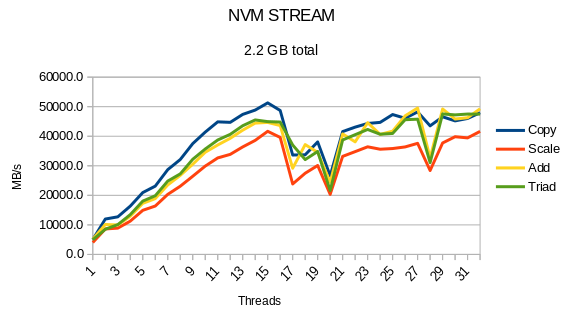
\includegraphics[scale=0.7]{Benchmarks/NVM_STREAM_100M_Figure.png}
\caption{NVDIMM Stream, 100,000,000 elements}
\label{fig:NVM_STREAM_100M_Figure}
\end{figure}

\begin{table}[!hbtp]
\begin{tabular}{ |c|c|c|c|c| } 
\hline
Threads & Copy & Scale & Add & Triad \\
\hline
1 & 5036.7 & 4026.4 & 5151.3 & 4956.0 \\
\hline
2 & 11970.2 & 8616.8 & 10120.7 & 8515.8 \\
\hline
3 & 12715.1 & 8903.4 & 9972.6 & 10085.0 \\
\hline
4 & 16349.6 & 11266.2 & 12922.7 & 13474.2 \\
\hline
5 & 20935.0 & 14924.3 & 17282.1 & 18050.7 \\
\hline
6 & 23119.7 & 16381.2 & 18887.2 & 19859.8 \\
\hline
7 & 28694.5 & 20320.0 & 23509.8 & 24824.9 \\
\hline
8 & 32104.6 & 23082.0 & 26744.5 & 27255.4 \\
\hline
9 & 37491.8 & 26450.3 & 30517.3 & 32194.4 \\
\hline
10 & 41394.8 & 29897.7 & 34575.6 & 35671.3 \\
\hline
11 & 44856.8 & 32659.1 & 37032.5 & 38714.6 \\
\hline
12 & 44695.1 & 33848.9 & 39292.6 & 40625.8 \\
\hline
13 & 47377.9 & 36377.7 & 42050.6 & 43542.1 \\
\hline
14 & 48853.3 & 38589.6 & 44440.4 & 45509.7 \\
\hline
15 & 51273.9 & 41662.3 & 44663.6 & 44941.4 \\
\hline
16 & 48704.8 & 39592.3 & 43615.7 & 44797.8 \\
\hline
17 & 33638.9 & 23842.9 & 29161.2 & 37024.5 \\
\hline
18 & 33712.5 & 27466.9 & 37166.7 & 32095.5 \\
\hline
19 & 38073.6 & 30095.0 & 34539.9 & 34835.6 \\
\hline
20 & 26627.1 & 20307.7 & 24445.4 & 21617.2 \\
\hline
21 & 41575.9 & 33180.5 & 40777.5 & 38727.8 \\
\hline
22 & 43078.1 & 34787.1 & 38100.6 & 40516.5 \\
\hline
23 & 44306.5 & 36409.9 & 44583.9 & 42289.1 \\
\hline
24 & 44679.1 & 35595.9 & 40602.3 & 40671.9 \\
\hline
25 & 47327.4 & 35824.6 & 41718.8 & 40939.5 \\
\hline
26 & 46085.6 & 36378.7 & 46893.2 & 45583.9 \\
\hline
27 & 48237.8 & 37579.8 & 49538.8 & 45762.3 \\
\hline
28 & 43507.7 & 28391.9 & 32673.6 & 31051.1 \\
\hline
29 & 46562.0 & 37710.1 & 49211.6 & 47533.4 \\
\hline
30 & 45188.7 & 39833.6 & 45820.8 & 47210.6 \\
\hline
31 & 46011.6 & 39429.2 & 46247.3 & 47491.9 \\
\hline
32 & 47961.6 & 41638.6 & 49278.3 & 47481.3 \\
\hline
\end{tabular}
\caption{NVDIMM Stream, 100,000,000 elements}
\label{tab:NVM_STREAM_100M_Table}
\end{table}

%\clearpage
\subsection{Competition benchmarks}
This chapter are about three different benchmarks. In the first benchmark data will be copied for a DRAM array to another DRAM array and from a NVDIMM array to another NVDIMM array simultaneously. In the second benchmark data will be copied from DRAM-DRAM arrays and from DRAM-NVDIMM arrays simultaneously. In the last benchmark data will be copied from DRAM-DRAM and NVDIMM-DRAM simultaneously.

The purpose of these benchmarks is to get an understanding of how performance will be affected when different threads generates traffic from DRAM and NVDIMM simultaneously. That is why there is three types of benchmarks in order to test all possible combination of traffic. Does a combination of DRAM and NVDIMM threads exist where the total bandwidth of DRAM and NVDIMM threads exceeds what a DRAM alone can archive. 

\subsubsection{NVM-NVM}
\label{section:NVM-NVM}
The code for this benchmark are described in listing \ref{lst:NVMNVMcode}.
From line 2-14 the code is declaring variables and creating the arrays where the result from the benchmark will be stored. There will be declared two DRAM array and two NVDIMM arrays that will be used in the benchmark.
When the threads arrive at line 16 they will synchronize before they are split into two group. Threads with a thread id lower than the number of DRAM threads will pass the if-sentence at line 17, where they will initiate two DRAM array and place values into each element.
The rest of the threads will move on to line 27 and enter this bracket. These threads will initiate two NVDIMM arrays and place values into each element.
All the threads will then synchronize at line 40 before they will divide into two group at line 41 in the same fashion they did in line 17. All the threads will then start to copy data from one array to the other array. The DRAM threads will copy from DRAM-DRAM array and the NVDIMM threads will copy from NVDIMM-NVDIMM array. They will repeat this for as many times as the user of the benchmark has decided by defining the total\_test variable as an argument in the command line when the program was started. The time measurement will be started at the beginning of the for-loop at line 45 or 54 and end at the end of the for-loop at line 50 or 60.
When the benchmark testing is over the threads will free up their arrays and the benchmark will print out the result. 

When the threads pass the barrier at line 40 and begin the benchmark test they will never synchronize another time. Because of this the DRAM threads will complete their tasks a lot earlier then NVDIMM threads because DRAM speed is faster then NVIDMM speed. This also means that once the fastest thread is done the rest of the threads will share more bandwidth among  themself and become faster. When more and more threads complete their tasks the faster the remaining threads will become.
In order to get a correct benchmark where all threads have been working the user need to throw out the data where some threads are working when other threads have completed their tasks. Throwing out the last one third is usually enough.
There is also a need to throw out atleast the first 25 iterations. This is because the NVDIMM is a lot slower to get started then DRAM. 

\begin{lstlisting}[caption={NVM-NVM source code},escapeinside={{/*!}{!*/}}, label={lst:NVMNVMcode}]
#pragma omp parallel
{
	//Declearing variables.
	int thread_id = omp_get_thread_num();
	int i,j;
	double *drm_read_array;
	double *drm_write_array;
	TOID(double) nvm_read_array;
	TOID(double) nvm_write_array;
	srand((unsigned int)time(NULL));	
	#pragma omp master
	{
		/* Creates array where the test result will be added. */
	}	
	//Creates all the arrays needed for the test.
	#pragma omp barrier
	if(thread_id < totalThreads-nvmThreads){
		drm_read_array = (double*)malloc(ARRAY_LENGTH*sizeof(double));
        drm_write_array = (double*)malloc(ARRAY_LENGTH*sizeof(double));
		#pragma omp critical
		{
			for(i=0;i<ARRAY_LENGTH;i++){
				drm_read_array[i] = ((double)rand()/(double)(RAND_MAX));
				drm_write_array[i] = ((double)rand()/(double)(RAND_MAX));
			}
		}
	}else if(thread_id >= totalThreads-nvmThreads){
		POBJ_ALLOC(pop, &nvm_read_array, double, sizeof(double) * ARRAY_LENGTH, NULL, NULL);
		POBJ_ALLOC(pop, &nvm_write_array, double, sizeof(double) * ARRAY_LENGTH, NULL, NULL);
		#pragma omp critical
		{
			for(i=0;i<ARRAY_LENGTH;i++){
				D_RW(nvm_read_array)[i] = ((double)rand()/(double)(RAND_MAX));
				D_RW(nvm_write_array)[i] = ((double)rand()/(double)(RAND_MAX));
			}
			//printf("NVM thread_id: %d, %f\n", thread_id, D_RO(nvm_read_array)[11235]);
		}
	}
	//Doing the test.
	#pragma omp barrier
	if(thread_id < totalThreads-nvmThreads){
		//From DRAM to DRAM:
		for(i=0;i<total_tests;i++){
			//Time start
			test_time[thread_id][i] = mysecond();
			for(j=0;j<ARRAY_LENGTH;j++){
				drm_write_array[j] = drm_read_array[j];
			}
			//Time stop.
			test_time[thread_id][i] = mysecond() - test_time[thread_id][i];
		}
	}else if(thread_id >= totalThreads-nvmThreads){
		//From NVM to NVM:
		for(i=0;i<total_tests;i++){
			//Time start
			test_time[thread_id][i] = mysecond2();
			for(j=0;j<ARRAY_LENGTH;j++)
				D_RW(nvm_write_array)[j] = D_RO(nvm_read_array)[j];
			//Time stop.
			test_time[thread_id][i] = mysecond2() - test_time[thread_id][i];
		}
	}else
		printf("ERROR\n");
	/* Freeing up DRAM and NVDIMM arrays */
}
\end{lstlisting}

%\clearpage
\begin{table}[!hbtp]
\begin{tabular}{ |c|c|c|c| } 
\hline
Threads & DRAM & NVDIMM & Sum \\
\hline
1 & 61042.84 & 3038.16 & 64081.01 \\
\hline
2 & 57761.80 & 6027.24 & 63789.03 \\
\hline
3 & 53767.10 & 9223.43 & 62990.52 \\
\hline
4 & 51257.79 & 12630.42 & 63888.22 \\
\hline
5 & 47770.89 & 15202.48 & 62973.37 \\
\hline
6 & 43771.07 & 18771.08 & 62542.15 \\
\hline
7 & 39780.16 & 22085.75 & 61865.90 \\
\hline
8 & 36275.70 & 25068.35 & 61344.05 \\
\hline
9 & 31873.99 & 28520.43 & 60394.42 \\
\hline
10 & 28691.82 & 30840.40 & 59532.22 \\
\hline
11 & 24580.59 & 33991.75 & 58572.33 \\
\hline
12 & 20550.17 & 38006.44 & 58556.61 \\
\hline
13 & 15877.24 & 40011.90 & 55889.14 \\
\hline
14 & 11010.71 & 43913.44 & 54924.15 \\
\hline
15 & 5932.95 & 46352.16 & 52285.11 \\
\hline
\end{tabular}
\caption{NVM-NVM, 32 GB}
\label{tab:NVM_NVM}
\end{table}

The Result of the benchmark is shown in figure \ref{fig:NVM_NVM} and table \ref{tab:NVM_NVM}. They show that as the number of NVDIMM threads increases at the expense of the DRAM threads the NVDIMM bandwidth increases and DRAM bandwidth decreases. 
The sum of the DRAM and NVDIMM start at 64,081 MB/s and decreases with 1,100 MB/s when there are five NVDIMM. When the number of NVDIMM threads increases even more, the bandwidth decreases at a  higher rate. From five to fifteen NVDIMM threads the bandwidth have decreased with 10,000 MB/s. This might be because the NVDIMM are not fast enough to make use of all the bandwidth that becomes available as the number of DRAM threads decreases. The result is that the user loses performance if the number of NVDIMM is too high.

\begin{figure}[!hbtp]
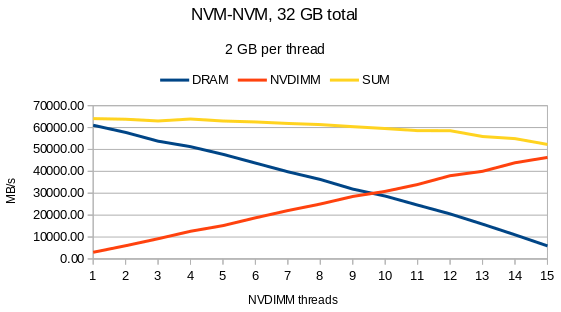
\includegraphics[scale=0.7]{Benchmarks/NVM-NVM_32GB_Figure.png}
\caption{NVM-NVM, 32 GB}
\label{fig:NVM_NVM}
\end{figure}

%\clearpage
%New graphs with second on x-axis and bandwidth on Y-axis. 500 iterations.
The graph in figure \ref{fig:NVM_NVM_sec} is the result of the same benchmark as figure \ref{fig:NVM_NVM}. The difference is that figure \ref{fig:NVM_NVM_sec} now show the number of seconds on x-axis and bandwidth on y-axis. Threads ends at different times. The last DRAM ends at 231 seconds and the last NVDIMM ends at around 319 seconds. The figure \ref{fig:NVM_NVM_sec} also show that all the DRAM threads have the same consistent speed except for the end of the DRAM. The NVDIMM threads on the other hand fluctuate a lot, they seem to have a speed at around 3,000 MB/s, but once in a while they drop down to 1,700 MB/s.
\begin{figure}[!hbtp]
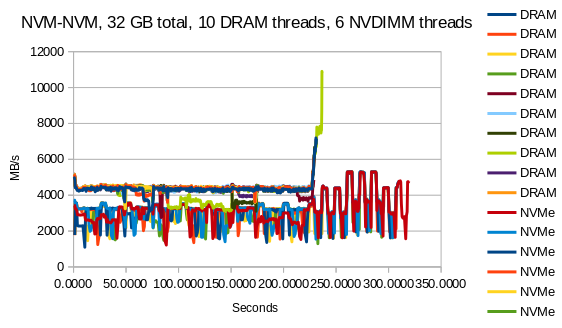
\includegraphics[scale=0.7]{Benchmarks/NVM-NVM_32GB_6_Thread.png}
\caption{NVM-NVM, 32 GB, 6 NVDIMM Threads}
\label{fig:NVM_NVM_sec}
\end{figure}

%\clearpage
\subsubsection{NVM-DRAM}
\label{section:NVM-DRAM}
In this version of the benchmark there will be one group of threads that transfer data from DRAM-DRAM and another group of threads that will transfer data from NVDIMM-DRAM. This code is very similar to the previous code. The differences are at line 26-36 where the code will initiate and add values to one DRAM array and one NVDIMM array instead of two NVDIMM arrays.  
The other difference is at line 51-61 where the code will copy data from NVDIMM-DRAM instead of NVDIMM-NVDIMM. 

\begin{lstlisting}[caption={NVM-DRAM source code},escapeinside={{/*!}{!*/}}]
#pragma omp parallel
{
	int thread_id = omp_get_thread_num();
	int i,j;
	double *drm_read_array;
	double *drm_write_array;
	TOID(double) nvm_read_array;
	srand((unsigned int)time(NULL));	
	#pragma omp master
	{
		/* Creates array where the test result will be added. */
	}
	//Creates all the arrays needed for the test.
	#pragma omp barrier
	if(thread_id < totalThreads-nvmThreads){
		drm_read_array = (double*)malloc(ARRAY_LENGTH*sizeof(double));
		drm_write_array = (double*)malloc(ARRAY_LENGTH*sizeof(double));
		#pragma omp critical
		{
			for(i=0;i<ARRAY_LENGTH;i++){
				drm_read_array[i] = ((double)rand()/(double)(RAND_MAX));
				drm_write_array[i] = ((double)rand()/(double)(RAND_MAX));
			}
		}
	}
	else if(thread_id >= totalThreads-nvmThreads){
		drm_write_array = (double*)malloc(ARRAY_LENGTH*sizeof(double));
		POBJ_ALLOC(pop, &nvm_read_array, double, sizeof(double) * ARRAY_LENGTH, NULL, NULL);
		#pragma omp critical
		{
			for(i=0;i<ARRAY_LENGTH;i++){
				D_RW(nvm_read_array)[i] = ((double)rand()/(double)(RAND_MAX));
				drm_write_array[i] = ((double)rand()/(double)(RAND_MAX));
			}
		}
	}
	//Doing the test.
	#pragma omp barrier
	if(thread_id < totalThreads-nvmThreads){
		//From DRAM to DRAM:
		for(i=0;i<total_tests;i++){
			//Time start
			test_time[thread_id][i] = mysecond();
			for(j=0;j<ARRAY_LENGTH;j++){
				drm_write_array[j] = drm_read_array[j];
			}
			//Time stop.
			test_time[thread_id][i] = mysecond() - test_time[thread_id][i];
		}
	}
	else if(thread_id >= totalThreads-nvmThreads){
		//From NVM to DRAM:
		for(i=0;i<total_tests;i++){
			//Time start
			test_time[thread_id][i] = mysecond();
			for(j=0;j<ARRAY_LENGTH;j++)
				drm_write_array[j] = D_RO(nvm_read_array)[j];
			//Time stop.
			test_time[thread_id][i] = mysecond() - test_time[thread_id][i];
		}
	}
	else
		printf("ERROR\n");
	/* Freeing up DRAM and NVDIMM arrays */
}
\end{lstlisting}

\begin{table}[!hbtp]
\begin{tabular}{ |c|c|c|c| } 
\hline
Threads & DRAM & NVDIMM & Sum \\
\hline
1 & 61257.14 & 3742.24 & 64999.37 \\
\hline
2 & 58419.89 & 6691.30 & 65111.18 \\
\hline
3 & 54544.07 & 10520.34 & 65064.41 \\
\hline
4 & 49997.69 & 15247.47 & 65245.16 \\
\hline
5 & 46226.88 & 19189.81 & 65416.69 \\
\hline
6 & 42942.39 & 22806.13 & 65748.52 \\
\hline
7 & 38156.47 & 27257.45 & 65413.92 \\
\hline
8 & 34613.22 & 30474.15 & 65087.37 \\
\hline
9 & 30458.70 & 34533.35 & 64992.05 \\
\hline
10 & 25489.86 & 39324.61 & 64814.47 \\
\hline
11 & 22083.85 & 42763.51 & 64847.36 \\
\hline
12 & 17704.90 & 47147.70 & 64852.60 \\
\hline
13 & 13394.67 & 51380.63 & 64775.31 \\
\hline
14 & 8947.75 & 56009.92 & 64957.67 \\
\hline
15 & 4489.12 & 60031.12 & 64520.24 \\
\hline
\end{tabular}
\caption{NVM-DRAM, 32 GB}
\label{tab:NVM_DRAM}
\end{table}

The result of this benchmark are shown in figure \ref{fig:NVM_DRAM} and table \ref{tab:NVM_DRAM}. Figure \ref{fig:NVM_DRAM} show that when the number of NVDIMM threads increases the NVDIMM bandwidth also goes up while the DRAM threads and bandwidth goes down. The sum of both the DRAM and NVDIMM bandwidth is stable at around 64,000 MB/s for all number of NVDIMM threads. 

\begin{figure}[!hbtp]
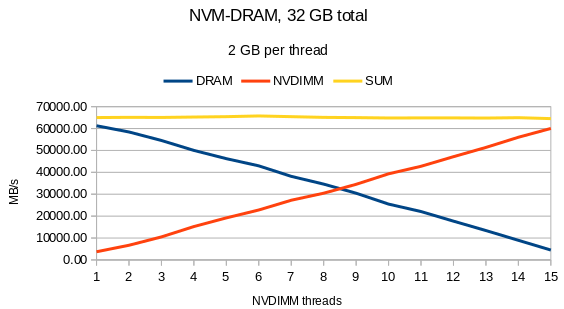
\includegraphics[scale=0.7]{Benchmarks/NVM-DRAM_32GB_Figure.png}
\caption{NVM-DRAM, 32 GB}
\label{fig:NVM_DRAM}
\end{figure}

Figure \ref{fig:NVM_DRAM_sec} shows the result of the same benchmark as figure \ref{fig:DRAM_NVM}, but with second on the x-axis. The last DRAM thread end at 234 seconds and the last NVDIMM thread end at 258 seconds. The DRAM threads consistent speed through the entire test at around 4,300 MB/s, only at the end will the speed increase because other threads have finished before them and therefore made more bandwidth available for the remaining threads. The NVDIMM threads are also more consistent in this benchmark where five of the six threads have speed of 3,800 MB/s for most of the test. There is only one thread that is fluctuating between 3,000 MB/s and 3,600 MB/s for most of the benchmark.

\begin{figure}[!hbtp]
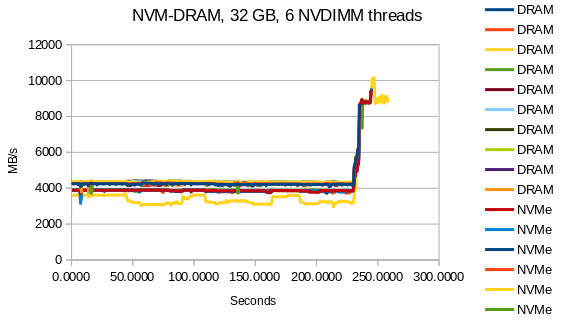
\includegraphics[scale=0.7]{Benchmarks/NVM-DRAM_32GB_6_Thread.png}
\caption{NVM-DRAM, 32 GB, 6 NVDIMM Threads}
\label{fig:NVM_DRAM_sec}
\end{figure}

\subsubsection{DRAM-NVM}
\label{section:DRAM-NVM}
In this version of the benchmark there will be one group of threads that transfer data from DRAM-DRAM and another group of threads that will transfer data from DRAM-NVDIMM. This code only have one difference when compared to the code in \ref{section:NVM-DRAM}. The difference is found in line 51-61 where data is transferred from DRAM-NVDIMM insted of from NVDIMM-DRAM.

\begin{lstlisting}[caption={DRAM-NVM source code},escapeinside={{/*!}{!*/}}]
#pragma omp parallel
{
	int thread_id = omp_get_thread_num();
	int i,j;
	double *drm_read_array;
	double *drm_write_array;
	TOID(double) nvm_write_array;
	srand((unsigned int)time(NULL));
	#pragma omp master
	{
		/* Creates array where the test result will be added. */
	}
	//Creates all the arrays needed for the test.
	#pragma omp barrier
	if(thread_id < totalThreads-nvmThreads){
		drm_read_array = (double*)malloc(ARRAY_LENGTH*sizeof(double));
    	drm_write_array = (double*)malloc(ARRAY_LENGTH*sizeof(double));
		#pragma omp critical
		{
			for(i=0;i<ARRAY_LENGTH;i++){
				drm_read_array[i] = ((double)rand()/(double)(RAND_MAX));
				drm_write_array[i] = ((double)rand()/(double)(RAND_MAX));
			}
		}
	}
	else if(thread_id >= totalThreads-nvmThreads){
		drm_read_array = (double*)malloc(ARRAY_LENGTH*sizeof(double));
    	POBJ_ALLOC(pop, &nvm_write_array, double, sizeof(double) * ARRAY_LENGTH, NULL, NULL);
		#pragma omp critical
		{
			for(i=0;i<ARRAY_LENGTH;i++){
				drm_read_array[i] = ((double)rand()/(double)(RAND_MAX));
				D_RW(nvm_write_array)[i] = ((double)rand()/(double)(RAND_MAX));
			}
		}
	}
	//Doing the test.
	#pragma omp barrier
	if(thread_id < totalThreads-nvmThreads){
		//From DRAM to DRAM:
		for(i=0;i<total_tests;i++){
			//Time start
			test_time[thread_id][i] = mysecond();	
			for(j=0;j<ARRAY_LENGTH;j++){
				drm_write_array[j] = drm_read_array[j];
			}
			//Time stop.
			test_time[thread_id][i] = mysecond() - test_time[thread_id][i];
		}
	}
	else if(thread_id >= totalThreads-nvmThreads){
		//From DRAM to NVM:
		for(i=0;i<total_tests;i++){
			//Time start
			test_time[thread_id][i] = mysecond();
			for(j=0;j<ARRAY_LENGTH;j++)
				D_RW(nvm_write_array)[j] = drm_read_array[j];		
			//Time stop.
			test_time[thread_id][i] = mysecond() - test_time[thread_id][i];
		}
	}
	else
		printf("ERROR\n");
	/* Freeing up DRAM and NVDIMM arrays */
}
\end{lstlisting}

%\clearpage
\begin{table}[!hbtp]
\begin{tabular}{ |c|c|c|c| }
\hline
Threads & DRAM & NVDIMM & Sum \\
\hline
1 & 61002.60 & 3581.48 & 64584.09 \\
\hline
2 & 56598.08 & 7323.96 & 63922.04 \\
\hline
3 & 53247.52 & 10954.06 & 64201.58 \\
\hline
4 & 48681.71 & 15070.61 & 63752.32 \\
\hline
5 & 44761.80 & 18725.90 & 63487.70 \\
\hline
6 & 41022.39 & 22614.45 & 63636.84 \\
\hline
7 & 36897.42 & 26557.71 & 63455.13 \\
\hline
8 & 32548.18 & 30570.88 & 63119.07 \\
\hline
9 & 28892.06 & 33996.95 & 62889.00 \\
\hline
10 & 24941.87 & 38191.10 & 63132.97 \\
\hline
11 & 20563.14 & 42263.28 & 62826.42 \\
\hline
12 & 16803.83 & 45915.39 & 62719.21 \\
\hline
13 & 12648.47 & 49341.90 & 61990.38 \\
\hline
14 & 8386.48 & 53331.10 & 61717.57 \\
\hline
15 & 4189.43 & 57348.14 & 61537.57 \\
\hline
\end{tabular}
\caption{DRAM-NVM, 32 GB}
\label{tab:DRAM_NVM}
\end{table}

The result of this benchmark are shown in figure \ref{fig:DRAM_NVM} and table \ref{tab:DRAM_NVM}. The result in figure \ref{fig:DRAM_NVM} is similar to the result in figure \ref{fig:NVM_DRAM} where NVDIMM speed increases and DRAM speed decreases at the same around the same rate. The sum of DRAM and NVDIMM speed remain stable at around 63,000 MB/s. Only at eleven NVDIMM threads and higher does the speed decrease a little. 

\begin{figure}[!hbtp]
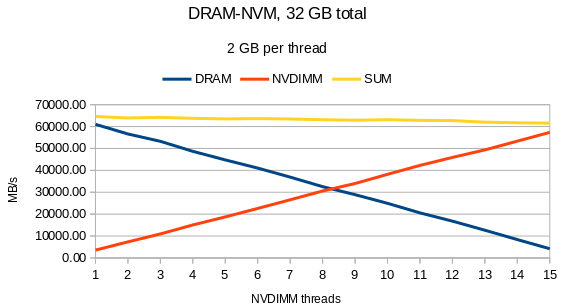
\includegraphics[scale=0.7]{Benchmarks/DRAM-NVM_32GB_Figure.png}
\caption{DRAM-NVM, 32 GB}
\label{fig:DRAM_NVM}
\end{figure}
%\clearpage
%New graphs with second on x-axis and bandwidth on Y-axis. 500 iterations.
Similar to to the other two benchmarks the DRAM threads in Figure \ref{fig:DRAM_NVM_sec} have more consistent speed than the NVDIMM. The speed of the DRAM threads are around 4,100 MB/s until the end where it increases sharply because other threads have completed their tasks and given the remaining threads more bandwidth. The speed of the NVDIMM is more unstable. The speed is remain at 3,800 MB/s, but all of the NVDIMM threads drops their speed several time during the test. Sometimes as low as 1,900 MB/s.

\begin{figure}[!hbtp]
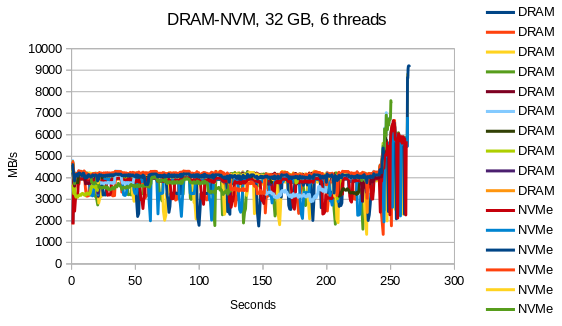
\includegraphics[scale=0.7]{Benchmarks/DRAM-NVM_32GB_6_Thread.png}
\caption{DRAM-NVM, 32 GB, 6 NVDIMM Threads}
\label{fig:DRAM_NVM_sec}
\end{figure}

\subsubsection{Observations}
\label{section:Observations}
The benchmarks at chapter \ref{section:NVM-DRAM} and chapter \ref{section:DRAM-NVM} have result more similar than the result in chapter \ref{section:NVM-NVM}. This is because the transfer speed DRAM to NVDIMM and NVDIMM to DRAM is almost identical. The DRAM-NVDIMM speed with one thread is 3581 MB/s and with fifteen thread the speed is 57348 MB/s. The NVDIMM-DRAM speed with one thread is 3742 an with fifteen thread the speed is 60031 MB/s. The speed with one and fifteen threads are almost the same. The rate the speed increase for each NVDIMM are also very similar.

The speed of the NVDIMM to NVDIMM in chapter \ref{section:NVM-NVM} is slower than than the other two benchmarks. When there is five threads the total speed of both DRAM and NVDIMM start to decrease and at fifteen threads the total speed have decreased by 10,000 MB/s. 
This means that if a program have two group of threads, one group only working on DRAM and the other only in NVDIMM. The program should not have more than five threads working on NVDIMM if the object is to maximize performance.

Figure \ref{fig:NVM_NVM_sec} in chapter \ref{section:NVM-NVM} and \ref{fig:DRAM_NVM_sec} in chapter \ref{section:DRAM-NVM} shows the NVDIMM threads fluctuate a lot. The figure in \ref{fig:NVM_DRAM_sec} in chapter \ref{section:NVM-DRAM} on the other hand show that all the NVDIMM threads except for one is a lot more stable. This might mean that writing to NVDIMM is a lot more sensitive to disturbances than what reading data from NVDIMM is.

The NVDIMM Stream in chapter \ref{section:STREAM_NVDIMM} also something similar where there are only NVDIMM threads and no traffic on DRAM. When each thread have their own core there is a smooth increase from one thread to sixteen threads. But when the hyper-treads are included and there are more than one thread per core the speed starts to fluctuate up and down for each new thread that is included.

Regardless of what the reason is for the fluctuations. The fluctuation might make it difficult to predict how much time it takes for an NVDIMM thread to complete a task.

%fra conclusion.
Table \ref{tab:Q1} show the copy speed of the two Stream benchmarks mentioned above. Table \ref{tab:Q1} end at sixteen threads while the Stream benchmarks test up to 32 threads. This is because the NVDIMM fluctuate too much to find a pattern. When the Stream is testing speed of only one thread the NVDIMM have a performance of 43\% of the speed of DRAM. When the number of threads increases the difference remain at around 40\% up until six threads. The exception to this is the test with two threads where the NVDIMM performance is 52\% of the DRAM performance.
The performance of NVDIMM at seven threads is at 51\% and when the number of threads increases the performance increases and end at 75\% when there is sixteen threads.

The reason the performance increases as more threads are added is because DRAM at 65,000 MB/s have reached the maximum capacity of the memory bandwidth. This allows the NVDIMM threads to catch up with the DRAM performance, but NVDIMM is only able to reach a performance 75\% of DRAM.

\begin{table}[!hbtp]
\begin{tabular}{ |c|c|c|c| }
\hline
Threads & DRAM & NVDIMM & Difference in \%\\
\hline
1 & 11673.5 & 5036.7 & 43.1 \\
\hline
2 & 22995.1 & 11970.2 & 52.1 \\
\hline
3 & 33554.9 & 12715.1 & 37.9 \\
\hline
4 & 42917.3 & 16349.6 & 38.1 \\
\hline
5 & 50260.9 & 20935.0 & 41.7 \\
\hline
6 & 53612.5 & 23119.7 & 43.1 \\
\hline
7 & 56100.8 & 28694.5 & 51.1 \\
\hline
8 & 58554.6 & 32104.6 & 54.8 \\
\hline
9 & 60491.7 & 37491.8 & 62.0 \\
\hline
10 & 62242.2 & 41394.8 & 66.5 \\
\hline
11 & 64257.1 & 44856.8 & 69.8 \\
\hline
12 & 64890.3 & 44695.1 & 68.9 \\
\hline
13 & 65648.8 & 47377.9 & 72.2 \\
\hline
14 & 65606.5 & 48853.3 & 74.5 \\
\hline
15 & 65665.5 & 51273.9 & 78.1 \\
\hline
16 & 65509.8 & 48704.8 & 74.3 \\
\hline
\end{tabular}
\caption{Difference in STREAM performance between DRAM and NVDIMM.}
\label{tab:Q1}
\end{table}


%\clearpage
\printbibliography


%%%%%%%%%%%%%%%%%%%%%%%%%%%%%%%%%%%%%%%%%%%%%%%%%%%%%%%%%%%
%		Kommentert ut skrift							  %
%%%%%%%%%%%%%%%%%%%%%%%%%%%%%%%%%%%%%%%%%%%%%%%%%%%%%%%%%%%



\begin{comment}
DRAM STREAM
\begin{table}[!hbtp]
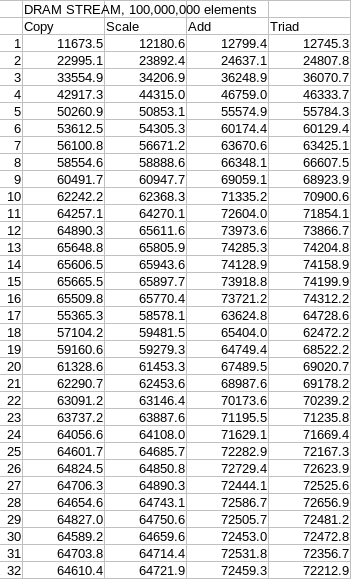
\includegraphics[scale=0.7]{Benchmarks/DRAM_STREAM_100M_Table.png}
\caption{DRAM Stream, 100,000,000 elements}
\end{table}
\begin{figure}[!hbtp]
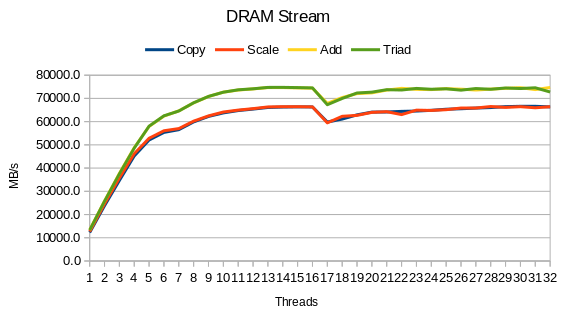
\includegraphics[scale=0.7]{DRAM_stream2.png}
\caption{DRAM Stream, Gammel}
\end{figure}
\end{comment}
\begin{comment}
NVM STREAM
\begin{table}[!hbtp]
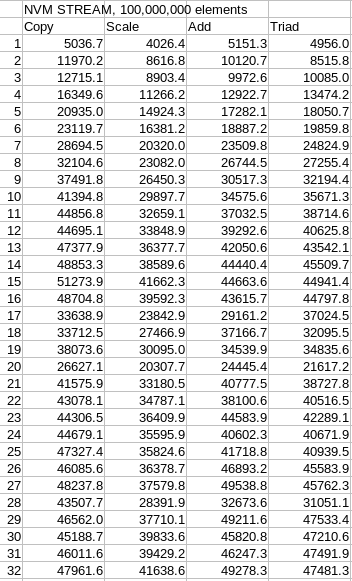
\includegraphics[scale=0.7]{Benchmarks/NVM_STREAM_100M_Table.png}
\caption{NVDIMM Stream, 100,000,000 elements}
\end{table}
\clearpage
\begin{table}[!hbtp]
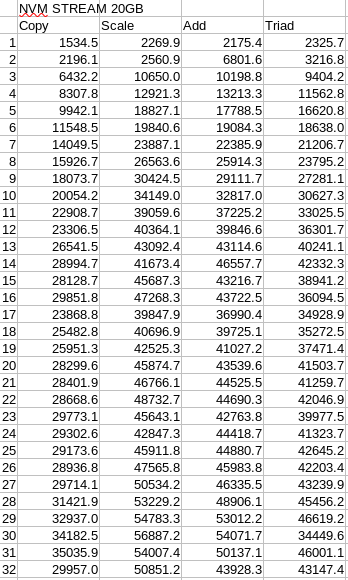
\includegraphics[scale=0.7]{Benchmarks/NVM_STREAM_14GB_Table_011121.png}
\caption{NVDIMM Stream, 2'000'000'000 elements}
\end{table}
\begin{figure}[!hbtp]
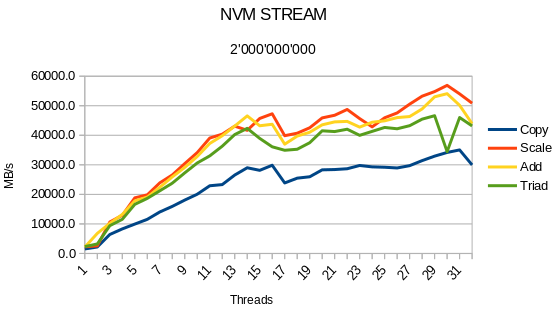
\includegraphics[scale=0.7]{Benchmarks/NVM_STREAM_14GB_Figure_011121.png}
\caption{NVDIMM Stream, 2'000'000'000 elements}
\end{figure}

\begin{figure}[!hbtp]
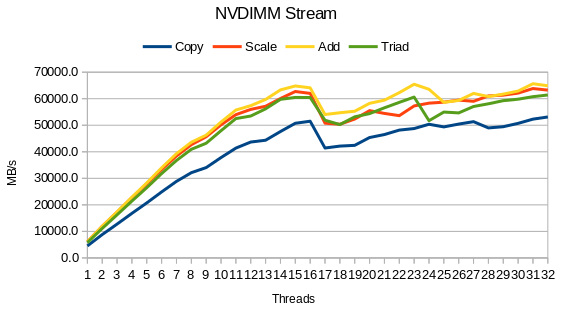
\includegraphics[scale=0.7]{NVDIMM_stream2.png}
\caption{NVDIMM Stream, Gammel måling}
\end{figure}
\end{comment}
\begin{comment}
STREAM NVM
Graphs and tables below show the speed of a certain amount of NVDIMM threads while the rest of the threads are from DRAM to DRAM.
The test have been conducted by transfer data simultaneously from DRAM-DRAM and NVM-NVM.
All the threads are transferring the values of one array to another, all the arrays have 100 million elements of type double. This transfer happens 5000 times and the graphs shows the average of the first 200 iterations. This is done to ensure that all the threads can't finish early and make the remaining threads faster. The sum graphs shows the sum bandwidth of DRAM and NVM. Average graphs shows the average bandwidth of DRAM and NVM.
\end{comment}
\begin{comment}
\subsubsection{The code}
The benchmark have three different program, the code is mostly the same except for the part where NVDIMM threads from NVDIMM-NVDIMM, DRAM-NVDIMM or NVDIMM-DRAM. 

The entire code is run in the main function except when it finds the current time, that is done in a different function.
The code begins with creating a memory pool and reads the parameters from command line. The parameters are how many threads are using the NVDIMM, the total amount of threads used and how many time the test will repeat itself. 
The code will then enter parallel area where one thread will create a 2d array where all the threads will save the time it took to copy the array. 

Every threads will then create their two arrays. The thread id will determine if both arrays will be DRAM array, or if one or two arrays will be NVDIMM array. Both arrays will be DRAM if the thread id is lower than the total amount of threads minus the number of NVDIMM threads. Thread ids equal or higher than that will either have one or both arrays stored in NVDIMM. All the arrays in all of the threads will be populated by random numbers. When a thread is done it will wait at a barrier until all the other threads are populating their threads.

\begin{lstlisting}[caption=Creation of DRAM and NVDIMM arrays]
if(thread_id < totalThreads-nvmThreads){
	//From DRAM to DRAM
	drm_read_array = (double*)malloc(ARRAY_LENGTH*sizeof(double));
	drm_write_array = (double*)malloc(ARRAY_LENGTH*sizeof(double));
	#pragma omp critical
	{
		for(i=0;i<ARRAY_LENGTH;i++){
			drm_read_array[i] = ((double)rand()/(double)(RAND_MAX));
			drm_write_array[i] = ((double)rand()/(double)(RAND_MAX));
		}
	}
}
else if(thread_id >= totalThreads-nvmThreads){
	//From NVDIMM to NVDIMM
	POBJ_ALLOC(pop, &nvm_read_array, double, sizeof(double) * ARRAY_LENGTH, NULL, NULL);
	POBJ_ALLOC(pop, &nvm_write_array, double, sizeof(double) * ARRAY_LENGTH, NULL, NULL);
	#pragma omp critical
	{
		for(i=0;i<ARRAY_LENGTH;i++){
			D_RW(nvm_read_array)[i] = ((double)rand()/(double)(RAND_MAX));
			D_RW(nvm_write_array)[i] = ((double)rand()/(double)(RAND_MAX));
		}
	}
}
\end{lstlisting}
%\label{testing}
%TESTING: /*!\ref{testing}!*/
Threads with DRAM arrays and threads with one or two NVDIMM array will split into their own part of the code with an if-sentence. All the threads will run the as many times as specified in the parameters and save the time each test takes in the 2d array that was created in the beginning. When they are done they will free up the memory and leave the parallel area. 

\begin{lstlisting}[caption=Threads running their test.]
if(thread_id < totalThreads-nvmThreads){
	//From DRAM to DRAM
	for(i=0;i<total_tests;i++){
		//Time start
		test_time[thread_id][i] = mysecond();
		for(j=0;j<ARRAY_LENGTH;j++){
			drm_write_array[j] = drm_read_array[j];
		}			
		//Time stop.
		test_time[thread_id][i] = mysecond() - test_time[thread_id][i];
	}
}
else if(thread_id >= totalThreads-nvmThreads){
	//From NVDIMM to NVDIMM
	for(i=0;i<total_tests;i++){
		//Time start
		test_time[thread_id][i] = mysecond2();
		for(j=0;j<ARRAY_LENGTH;j++)
			D_RW(nvm_write_array)[j] = D_RO(nvm_read_array)[j];		
		//Time stop.
		test_time[thread_id][i] = mysecond2() - test_time[thread_id][i];
	}
}
\end{lstlisting}

The code will then print the entire 2d array where the time measurements are stored to the terminal. Each line represent all the test done by one thread. In the beginning of each line the code will add either DRAM if both arrays are stored on DRAM. Or NVM if one or both arrays are stored on NVDIMM. When the program is done printing it will exit.
\end{comment}
\begin{comment}
under NVM-NVM
\begin{table}[!hbtp]
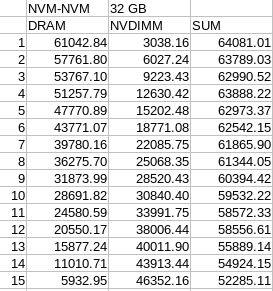
\includegraphics[scale=0.7]{Benchmarks/NVM-NVM_32GB_Table.png}
\caption{NVM-NVM, 32 GB}
\end{table}
\begin{table}[!hbtp]
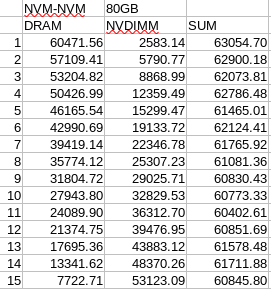
\includegraphics[scale=0.7]{Benchmarks/NVM-NVM_80GB_Table.png}
\caption{NVM-NVM, 80 GB}
\end{table}
\begin{figure}[!hbtp]
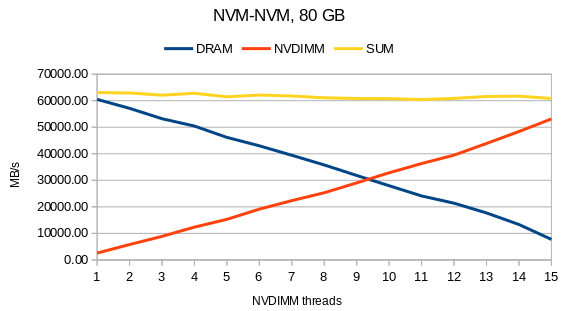
\includegraphics[scale=0.7]{Benchmarks/NVM-NVM_80GB_Figure.png}
\caption{NVM-NVM, 80 GB}
\end{figure}
Gammelt? \\
The tables below shows the result of the benchmark where one group of threads transfer from DRAM-DRAM and another group from NVDIMM-NVDIMM. The test result in the tables are the transfer speed in MB/s. The first table shows the combined transfer speed of all threads that are copying from DRAM-DRAM and the second table shows the combined speed of all the threads that are copying from NVDIMM-NVDIMM. 

The first line in the first table in figure 2 shows the combined transfer speed of the DRAM-DRAM copying where there are one thread copying from NVDIMM-NVDIMM. That means there are 15 threads that are copying from DRAM-DRAM. 
The first line in the second table shows the transfer speed of that one thread. The columns shows the the test numbers. The column with name the "1-20" shows the average transfer speed of the first 20 tests.
The third table in figure 3 shows the combined transfer speed of all the 16 threads in the first two tables. 
There is also a graph where all three tables are being represented.

One of the hopes by using NVDIMM and DRAM simultaneously was that there would be an increase in the transfer speed. But by comparing copy on figure 1 with the sum on figure 4 one can see that there has been no increase in transfer speed. Both graphs shows a transfer speed on around 65000 MB/s.
\begin{figure}[!hbtp]
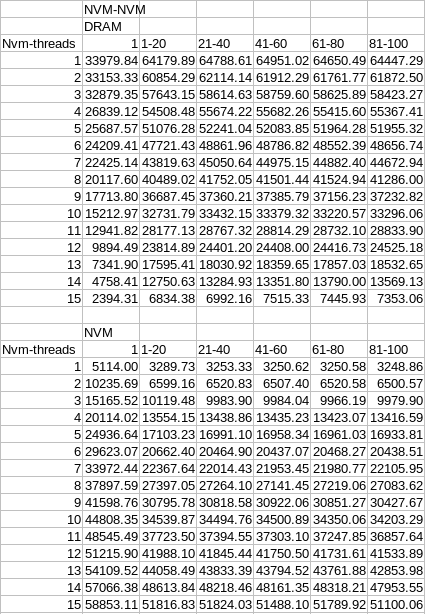
\includegraphics[scale=0.7]{NVM-NVM_table_p1_1-100_v3}
\caption{NVM-NVM 1-100 iteration, 16 threads total, 3rd version}
\end{figure}
\begin{figure}[!hbtp]
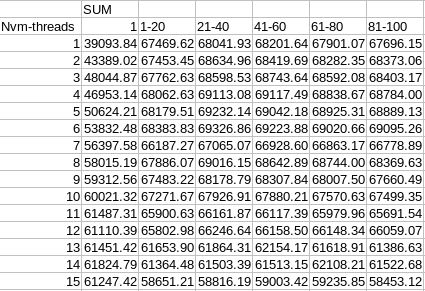
\includegraphics[scale=0.7]{NVM-NVM_table_p2_1-100_v3}
\caption{NVM-NVM 1-100 iteration, 16 threads total, 3rd version}
\end{figure}
\begin{figure}[!hbtp]
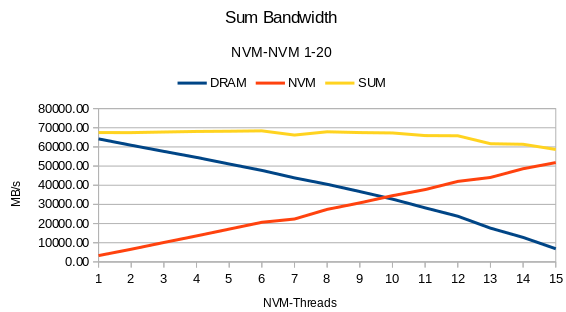
\includegraphics[scale=0.7]{NVM-NVM_Graph_1-20_v3}
\caption{NVM-NVM graph 1-20, 3rd version}
\end{figure}
\end{comment}
\begin{comment}
UNDER NVM-DRAM
\begin{table}[!hbtp]
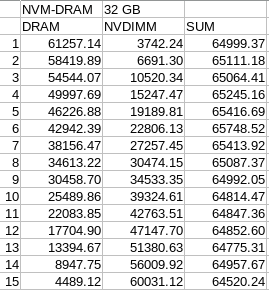
\includegraphics[scale=0.7]{Benchmarks/NVM-DRAM_32GB_Table.png}
\caption{NVM-DRAM, 32 GB}
\end{table}
This benchmark is similar to the previous benchmark. The only difference is that some threads will transfer data from NVDIMM-DRAM instead of NVDIMM-NVDIMM.
\begin{figure}[!hbtp]
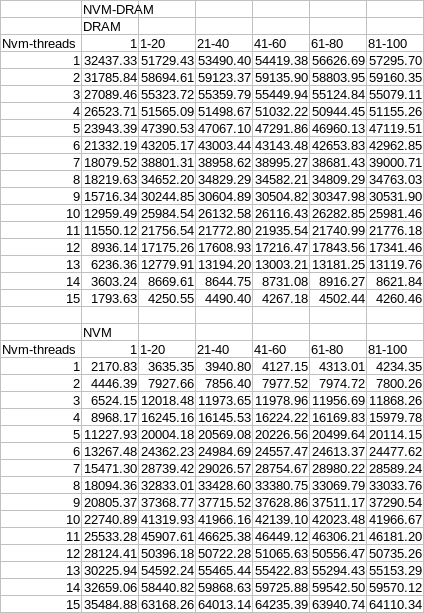
\includegraphics[scale=0.7]{NVM-DRAM_table_p1_1-100_v3}
\caption{NVM-DRAM 1-100 iteration, 3rd version}
\end{figure}

\begin{figure}[!hbtp]
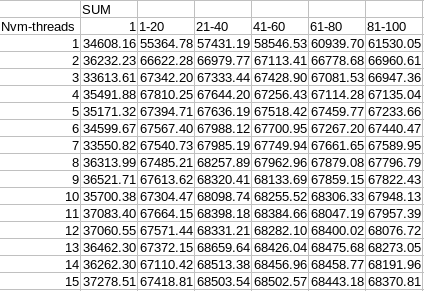
\includegraphics[scale=0.7]{NVM-DRAM_table_p2_1-100_v3}
\caption{NVM-DRAM 1-100 iteration, 3rd version}
\end{figure}

\begin{figure}[!hbtp]
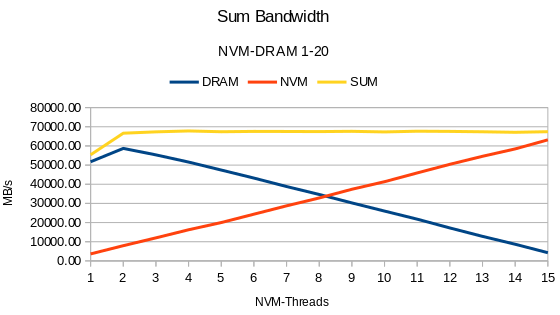
\includegraphics[scale=0.7]{NVM-DRAM_Graph_1-20_v3}
\caption{NVM-DRAM graph 1-20, 3rd version}
\end{figure}
\end{comment}
\begin{comment}
UNDER DRAM-NVM
\begin{table}[!hbtp]
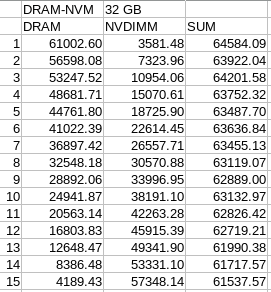
\includegraphics[scale=0.7]{Benchmarks/DRAM-NVM_32GB_Table.png}
\caption{DRAM-NVM, 32 GB}
\end{table}
This benchmark is also similar to the other two benchmarks. This time some of the threads will transfer from DRAM-NVDIMM.
\begin{figure}[!hbtp]
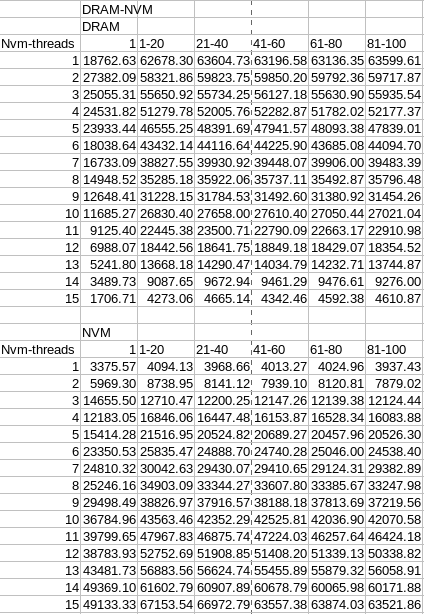
\includegraphics[scale=0.7]{DRAM-NVM_table_p1_1-100_v3}
\caption{DRAM-NVM 1-100 iteration, 3rd version}
\end{figure}

\begin{figure}[!hbtp]
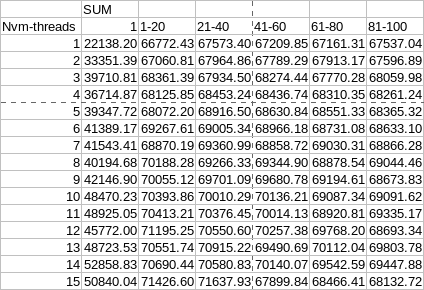
\includegraphics[scale=0.7]{DRAM-NVM_table_p2_1-100_v3}
\caption{DRAM-NVM 1-100 iteration, 3rd version}
\end{figure}

\begin{figure}[!hbtp]
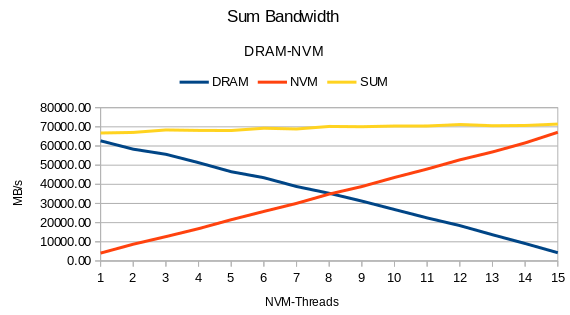
\includegraphics[scale=0.7]{DRAM-NVM_Graph_1-20_v3}
\caption{DRAM-NVM graph 1-20, 3rd version}
\end{figure}
\end{comment}
\end{document}               % End of document.
